\documentclass[11pt,a4paper]{article}
\usepackage[utf8]{vietnam}
\usepackage{amsmath,amssymb}
\usepackage{tabularx}
\usepackage{tikz}
\usepackage{xcolor}
\usepackage{fancyhdr}
\usepackage[top=1.8cm, bottom=2.0cm, left=1.8cm, right=1.8cm]{geometry}

\setlength{\parskip}{3pt}
\setlength{\parindent}{0pt}

\pagestyle{fancy}
\fancyhf{}
\renewcommand{\headrulewidth}{0.4pt}
\lhead{\footnotesize \textbf{CHÙA HƯƠNG SƠN -- ÔN THI VÀO 10}}
\rhead{\footnotesize \textbf{ĐỀ THI THỬ CUỐI HỌC KỲ I (ĐỀ SỐ 02)}}
\cfoot{\thepage}

\begin{document}

\noindent
\begin{tabular*}{\linewidth}{@{\extracolsep{\fill}}cc@{}}
\textbf{SỞ GIÁO DỤC VÀ ĐÀO TẠO} & \textbf{ĐỀ KIỂM TRA CUỐI HỌC KỲ I} \\
\textbf{CHÙA HƯƠNG SƠN} & \textbf{NĂM HỌC 2026 -- 2027} \\
\textbf{ĐỀ THI THỬ SỐ 02} & \textbf{MÔN: TOÁN -- LỚP 9} \\
\textit{(Đề thi gồm 03 trang)} & \textit{Thời gian làm bài: 90 phút (không kể thời gian phát đề)} \\
\end{tabular*}

\vspace{2mm}
\noindent
\rule{\linewidth}{0.8pt}

\vspace{1mm}
\noindent
Họ và tên thí sinh: \dotfill Số báo danh: \dotfill

\vspace{2mm}
\noindent
\textbf{\large I. TRẮC NGHIỆM KHÁCH QUAN (7,0 điểm)}

\vspace{1mm}
\noindent
\textbf{Phần 1. Trắc nghiệm nhiều lựa chọn (3,0 điểm).} \textit{Từ câu 1 đến câu 12, thí sinh chọn đáp án đúng nhất trong 4 đáp án A, B, C, D rồi ghi vào bài làm.}

\vspace{1.5mm}
\textbf{Câu 1.} Giá trị của biểu thức $2\sqrt{27} - 3\sqrt{12} + \sqrt{75}$ bằng\\
\begin{tabularx}{\linewidth}{XXXX}
\textbf{A.} $5\sqrt{3}$. & \textbf{B.} $-5\sqrt{3}$. & \textbf{C.} $3\sqrt{3}$. & \textbf{D.} $0$.
\end{tabularx}

\vspace{1.5mm}
\textbf{Câu 2.} Cho tam giác $DEF$ vuông tại $D$, góc nhọn $\widehat{F} = \alpha$. Khẳng định nào sau đây là đúng?\\
\begin{tabularx}{\linewidth}{XXXX}
\textbf{A.} $\sin \alpha = \dfrac{DE}{EF}$. & \textbf{B.} $\cos \alpha = \dfrac{DE}{EF}$. & \textbf{C.} $\tan \alpha = \dfrac{DF}{DE}$. & \textbf{D.} $\cot \alpha = \dfrac{DE}{DF}$.
\end{tabularx}

\vspace{1.5mm}
\textbf{Câu 3.} Bất phương trình nào sau đây là bất phương trình bậc nhất một ẩn?\\
\begin{tabularx}{\linewidth}{XXXX}
\textbf{A.} $x^2 - 4 \le 0$. & \textbf{B.} $0x + 8 > 0$. & \textbf{C.} $-3x + 9 \ge 0$. & \textbf{D.} $\dfrac{1}{x} + 2 < 0$.
\end{tabularx}

\vspace{1.5mm}
\textbf{Câu 4.} Nếu $x > y$ thì bất đẳng thức nào sau đây luôn đúng?\\
\begin{tabularx}{\linewidth}{XXXX}
\textbf{A.} $-2x < -2y$. & \textbf{B.} $-2x > -2y$. & \textbf{C.} $x - 3 < y - 3$. & \textbf{D.} $3x + 1 < 3y + 1$.
\end{tabularx}

\vspace{1.5mm}
\textbf{Câu 5.} Căn bậc hai số học của số 100 là\\
\begin{tabularx}{\linewidth}{XXXX}
\textbf{A.} $10$ và $-10$. & \textbf{B.} $10$. & \textbf{C.} $-10$. & \textbf{D.} $50$.
\end{tabularx}

\vspace{1.5mm}
\textbf{Câu 6.} Điều kiện xác định của căn thức $\sqrt{3x - 12}$ là\\
\begin{tabularx}{\linewidth}{XXXX}
\textbf{A.} $x \ge 4$. & \textbf{B.} $x > 4$. & \textbf{C.} $x \le 4$. & \textbf{D.} $x < 4$.
\end{tabularx}

\vspace{1.5mm}
\textbf{Câu 7.} Với mọi số thực $x < 2$, giá trị của biểu thức $\sqrt{(x-2)^2}$ bằng\\
\begin{tabularx}{\linewidth}{XXXX}
\textbf{A.} $x - 2$. & \textbf{B.} $2 - x$. & \textbf{C.} $-(2-x)$. & \textbf{D.} $(x-2)^2$.
\end{tabularx}

\vspace{1.5mm}
\textbf{Câu 8.} Giá trị của $\sqrt[3]{-216}$ bằng\\
\begin{tabularx}{\linewidth}{XXXX}
\textbf{A.} $6$. & \textbf{B.} $-6$. & \textbf{C.} $36$. & \textbf{D.} $-36$.
\end{tabularx}

\vspace{1.5mm}
\textbf{Câu 9.} Trong đường tròn $(O; R)$, công thức tính chu vi (độ dài) của đường tròn là\\
\begin{tabularx}{\linewidth}{XXXX}
\textbf{A.} $C = 2\pi R$. & \textbf{B.} $C = \pi R$. & \textbf{C.} $C = \pi R^2$. & \textbf{D.} $C = 2\pi R^2$.
\end{tabularx}

\vspace{1.5mm}
\textbf{Câu 10.} Cho đường tròn $(O; 4\text{ cm})$ và đường thẳng $a$. Biết khoảng cách từ $O$ đến $a$ là $3\text{ cm}$. Vị trí tương đối của đường thẳng $a$ và đường tròn $(O)$ là\\
\begin{tabularx}{\linewidth}{XXXX}
\textbf{A.} Tiếp xúc nhau. & \textbf{B.} Cắt nhau. & \textbf{C.} Không giao nhau. & \textbf{D.} Trùng nhau.
\end{tabularx}

\vspace{1.5mm}
\textbf{Câu 11.} Cho hai đường tròn $(O; 6\text{ cm})$ và $(O'; 2\text{ cm})$. Biết khoảng cách giữa hai tâm $OO' = 8\text{ cm}$. Vị trí tương đối của hai đường tròn $(O)$ và $(O')$ là\\
\begin{tabularx}{\linewidth}{XXXX}
\textbf{A.} Tiếp xúc ngoài. & \textbf{B.} Tiếp xúc trong. & \textbf{C.} Cắt nhau. & \textbf{D.} Ở ngoài nhau.
\end{tabularx}

\vspace{1.5mm}
\textbf{Câu 12.} Trên đường tròn $(O)$, cho góc ở tâm $\widehat{COD} = 110^\circ$. Số đo của cung nhỏ $CD$ bằng\\
\begin{tabularx}{\linewidth}{XXXX}
\textbf{A.} $55^\circ$. & \textbf{B.} $220^\circ$. & \textbf{C.} $110^\circ$. & \textbf{D.} $70^\circ$.
\end{tabularx}

\vspace{3mm}
\noindent
\textbf{Phần 2. Trắc nghiệm Đúng -- Sai (2,0 điểm).} \textit{Trong mỗi ý a), b), c), d) ở câu 13 và câu 14, thí sinh chọn đúng hoặc sai và ghi chữ ``Đ'' hoặc ``S'' vào bài làm.}

\vspace{1.5mm}
\textbf{Câu 13.} Xét bài toán thực tế: ``Quãng đường $AB$ dài $180\text{ km}$. Lúc 7 giờ sáng, một ô tô khởi hành từ $A$ đi về $B$ với vận tốc $50\text{ km/h}$. Cùng lúc đó, một xe máy khởi hành từ $B$ đi về $A$ với vận tốc $40\text{ km/h}$. Coi hai xe chuyển động thẳng đều trên đoạn đường $AB$.''\\
Xét tính đúng sai của các khẳng định sau:
\begin{center}
\begin{tabularx}{\linewidth}{|X|c|c|}
\hline
\textbf{Khẳng định} & \textbf{Đúng} & \textbf{Sai} \\
\hline
a) Sau 1 giờ kể từ lúc khởi hành, ô tô đi được quãng đường là $50\text{ km}$. & & \\
\hline
b) Hai xe gặp nhau tại thời điểm lúc 9 giờ sáng cùng ngày. & & \\
\hline
c) Địa điểm hai xe gặp nhau cách điểm $A$ một khoảng là $80\text{ km}$. & & \\
\hline
d) Sau 1,5 giờ kể từ lúc khởi hành, khoảng cách giữa hai xe là $45\text{ km}$. & & \\
\hline
\end{tabularx}
\end{center}

\vspace{2mm}
\textbf{Câu 14.} Cho đường tròn $(O; 5\text{ cm})$ và dây cung $AB = 8\text{ cm}$ không đi qua tâm $O$. Qua $O$ kẻ đường thẳng vuông góc với $AB$ tại $H$, đường thẳng này cắt tiếp tuyến tại $A$ của đường tròn $(O)$ tại điểm $C$.\\
Xét tính đúng sai của các khẳng định sau:
\begin{center}
\begin{tabularx}{\linewidth}{|X|c|c|}
\hline
\textbf{Khẳng định} & \textbf{Đúng} & \textbf{Sai} \\
\hline
a) Điểm $H$ là trung điểm của đoạn thẳng $AB$ và $AH = 4\text{ cm}$. & & \\
\hline
b) Khoảng cách từ tâm $O$ đến dây cung $AB$ là $OH = 3\text{ cm}$. & & \\
\hline
c) Đoạn thẳng $CB$ là tiếp tuyến của đường tròn $(O)$. & & \\
\hline
d) Độ dài đoạn thẳng $OC$ bằng $8\text{ cm}$. & & \\
\hline
\end{tabularx}
\end{center}

\vspace{3mm}
\noindent
\textbf{Phần 3. Trắc nghiệm trả lời ngắn (2,0 điểm).} \textit{Từ câu 15 đến câu 18, thí sinh chỉ ghi kết quả cuối cùng vào bài làm.}

\vspace{1.5mm}
\textbf{Câu 15.} Nghiệm của bất phương trình $2(x - 3) + 7 < 3(x + 1) - 4$ là $\dots\dots\dots$

\vspace{1.5mm}
\textbf{Câu 16.} Giá trị của biểu thức $M = \sqrt{(\sqrt{5} - 3)^2} + \sqrt{5}$ bằng $\dots\dots\dots$

\vspace{1.5mm}
\noindent
\begin{minipage}[c]{0.65\linewidth}
\textbf{Câu 17.} Từ đỉnh một ngọn hải đăng cao $50\text{ m}$ so với mực nước biển, một người quan sát nhìn thấy một con tàu dưới một góc hạ $30^\circ$ so với phương nằm ngang (xem hình vẽ bên). Hỏi khoảng cách từ chân ngọn hải đăng đến con tàu là bao nhiêu mét? (làm tròn kết quả đến hàng phần mười của mét).
\end{minipage}\hfill
\begin{minipage}[c]{0.32\linewidth}
\centering
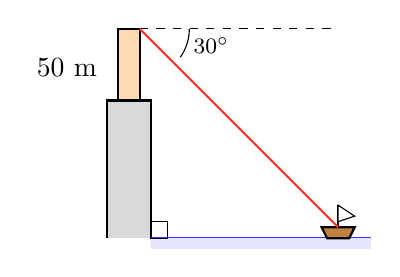
\begin{tikzpicture}[scale=0.7]
  % Vách đá và hải đăng
  \fill[gray!30] (0,0) -- (0,2.5) -- (0.8,2.5) -- (0.8,0) -- cycle;
  \draw[thick] (0,0) -- (0,2.5) -- (0.8,2.5) -- (0.8,0);
  % Ngọn hải đăng
  \draw[thick, fill=orange!30] (0.2,2.5) rectangle (0.6,3.8);
  \node[left] at (0, 3.1) {$50\text{ m}$};
  % Mực nước biển
  \draw[thick, blue!80] (0.8,0) -- (4.8,0);
  \fill[blue!10] (0.8,-0.2) rectangle (4.8,0);
  % Con thuyền
  \draw[thick, fill=brown] (4.0,0) -- (4.4,0) -- (4.5,0.2) -- (3.9,0.2) -- cycle;
  \draw[thick] (4.2,0.2) -- (4.2,0.6);
  \draw[fill=white] (4.2,0.3) -- (4.5,0.4) -- (4.2,0.6) -- cycle;
  % Tia quan sát và phương ngang
  \draw[dashed] (0.6,3.8) -- (4.2,3.8);
  \draw[thick, red!80] (0.6,3.8) -- (4.2,0.2);
  \draw (1.5,3.8) arc (0:-35:0.9);
  \node at (1.9, 3.5) {\footnotesize $30^\circ$};
  % Góc vuông
  \draw (0.8,0) rectangle (1.1,0.3);
\end{tikzpicture}
\end{minipage}

\vspace{1.5mm}
\textbf{Câu 18.} Một chiếc bánh pizza hình tròn có bán kính $R = 18\text{ cm}$ được cắt thành 8 miếng bằng nhau hình quạt tròn. Tính diện tích bề mặt của một miếng bánh pizza đó (lấy $\pi \approx 3{,}14$, làm tròn kết quả đến hàng phần mười, đơn vị: $\text{cm}^2$).

\vspace{4mm}
\noindent
\textbf{\large II. TỰ LUẬN (3,0 điểm).} \textit{Thí sinh trình bày lời giải chi tiết vào tờ giấy thi.}

\vspace{2mm}
\textbf{Câu 19 (1,0 điểm).}
\begin{itemize}
  \item[a)] \textit{(0,5 điểm)} Giải hệ phương trình: $\begin{cases} 2x - 3y = 1 \\ 3x + 2y = 8 \end{cases}$.
  \item[b)] \textit{(0,5 điểm)} Cho biểu thức $B = \left( \dfrac{\sqrt{x}}{\sqrt{x}-2} - \dfrac{4}{x - 2\sqrt{x}} \right) : \dfrac{\sqrt{x}+2}{\sqrt{x}}$ với $x > 0, x \ne 4$. Rút gọn biểu thức $B$.
\end{itemize}

\vspace{2mm}
\textbf{Câu 20 (1,5 điểm).} Cho đường tròn $(O; R)$ và dây cung $AB$ không đi qua tâm $O$. Qua $O$ kẻ đường thẳng vuông góc với $AB$ tại $H$, đường thẳng này cắt tiếp tuyến tại $A$ của đường tròn $(O)$ tại điểm $C$.
\begin{itemize}
  \item[a)] \textit{(0,75 điểm)} Chứng minh rằng đường thẳng $CB$ là tiếp tuyến của đường tròn $(O)$.
  \item[b)] \textit{(0,75 điểm)} Cho biết bán kính $R = 5\text{ cm}$ và dây cung $AB = 8\text{ cm}$. Tính độ dài đoạn thẳng $OC$ và $AC$.
\end{itemize}

\vspace{2mm}
\textbf{Câu 21 (0,5 điểm).}
\begin{itemize}
  \item[a)] \textit{(0,25 điểm)} Một bể bơi không nắp có dạng hình hộp chữ nhật với đáy là hình vuông, có thể tích bằng $32\text{ m}^3$. Người ta cần lát gạch men toàn bộ mặt đáy và bốn mặt xung quanh bên trong bể. Hãy xác định kích thước cạnh đáy và chiều sâu của bể để tổng diện tích gạch lát cần dùng là nhỏ nhất (nhằm tiết kiệm chi phí thi công nhất).
  \item[b)] \textit{(0,25 điểm)} Cho ba số thực dương $a, b, c$ thỏa mãn điều kiện $a + b + c = 6$. Tìm giá trị nhỏ nhất của biểu thức:
  \[
  P = \dfrac{1}{a} + \dfrac{4}{b} + \dfrac{9}{c}.
  \]
\end{itemize}

\vspace{4mm}
\begin{center}
\textbf{---------- HẾT ----------}\\
\textit{(Cán bộ coi thi không giải thích gì thêm)}
\end{center}

\end{document}
